\documentclass[1p]{elsarticle_modified}
%\bibliographystyle{elsarticle-num}

%\usepackage[colorlinks]{hyperref}
%\usepackage{abbrmath_seonhwa} %\Abb, \Ascr, \Acal ,\Abf, \Afrak
\usepackage{amsfonts}
\usepackage{amssymb}
\usepackage{amsmath}
\usepackage{amsthm}
\usepackage{scalefnt}
\usepackage{amsbsy}
\usepackage{kotex}
\usepackage{caption}
\usepackage{subfig}
\usepackage{color}
\usepackage{graphicx}
\usepackage{xcolor} %% white, black, red, green, blue, cyan, magenta, yellow
\usepackage{float}
\usepackage{setspace}
\usepackage{hyperref}

\usepackage{tikz}
\usetikzlibrary{arrows}

\usepackage{multirow}
\usepackage{array} % fixed length table
\usepackage{hhline}

%%%%%%%%%%%%%%%%%%%%%
\makeatletter
\renewcommand*\env@matrix[1][\arraystretch]{%
	\edef\arraystretch{#1}%
	\hskip -\arraycolsep
	\let\@ifnextchar\new@ifnextchar
	\array{*\c@MaxMatrixCols c}}
\makeatother %https://tex.stackexchange.com/questions/14071/how-can-i-increase-the-line-spacing-in-a-matrix
%%%%%%%%%%%%%%%

\usepackage[normalem]{ulem}

\newcommand{\msout}[1]{\ifmmode\text{\sout{\ensuremath{#1}}}\else\sout{#1}\fi}
%SOURCE: \msout is \stkout macro in https://tex.stackexchange.com/questions/20609/strikeout-in-math-mode

\newcommand{\cancel}[1]{
	\ifmmode
	{\color{red}\msout{#1}}
	\else
	{\color{red}\sout{#1}}
	\fi
}

\newcommand{\add}[1]{
	{\color{blue}\uwave{#1}}
}

\newcommand{\replace}[2]{
	\ifmmode
	{\color{red}\msout{#1}}{\color{blue}\uwave{#2}}
	\else
	{\color{red}\sout{#1}}{\color{blue}\uwave{#2}}
	\fi
}

\newcommand{\Sol}{\mathcal{S}} %segment
\newcommand{\D}{D} %diagram
\newcommand{\A}{\mathcal{A}} %arc


%%%%%%%%%%%%%%%%%%%%%%%%%%%%%5 test

\def\sl{\operatorname{\textup{SL}}(2,\Cbb)}
\def\psl{\operatorname{\textup{PSL}}(2,\Cbb)}
\def\quan{\mkern 1mu \triangleright \mkern 1mu}

\theoremstyle{definition}
\newtheorem{thm}{Theorem}[section]
\newtheorem{prop}[thm]{Proposition}
\newtheorem{lem}[thm]{Lemma}
\newtheorem{ques}[thm]{Question}
\newtheorem{cor}[thm]{Corollary}
\newtheorem{defn}[thm]{Definition}
\newtheorem{exam}[thm]{Example}
\newtheorem{rmk}[thm]{Remark}
\newtheorem{alg}[thm]{Algorithm}

\newcommand{\I}{\sqrt{-1}}
\begin{document}

%\begin{frontmatter}
%
%\title{Boundary parabolic representations of knots up to 8 crossings}
%
%%% Group authors per affiliation:
%\author{Yunhi Cho} 
%\address{Department of Mathematics, University of Seoul, Seoul, Korea}
%\ead{yhcho@uos.ac.kr}
%
%
%\author{Seonhwa Kim} %\fnref{s_kim}}
%\address{Center for Geometry and Physics, Institute for Basic Science, Pohang, 37673, Korea}
%\ead{ryeona17@ibs.re.kr}
%
%\author{Hyuk Kim}
%\address{Department of Mathematical Sciences, Seoul National University, Seoul 08826, Korea}
%\ead{hyukkim@snu.ac.kr}
%
%\author{Seokbeom Yoon}
%\address{Department of Mathematical Sciences, Seoul National University, Seoul, 08826,  Korea}
%\ead{sbyoon15@snu.ac.kr}
%
%\begin{abstract}
%We find all boundary parabolic representation of knots up to 8 crossings.
%
%\end{abstract}
%\begin{keyword}
%    \MSC[2010] 57M25 
%\end{keyword}
%
%\end{frontmatter}

%\linenumbers
%\tableofcontents
%
\newcommand\colored[1]{\textcolor{white}{\rule[-0.35ex]{0.8em}{1.4ex}}\kern-0.8em\color{red} #1}%
%\newcommand\colored[1]{\textcolor{white}{ #1}\kern-2.17ex	\textcolor{white}{ #1}\kern-1.81ex	\textcolor{white}{ #1}\kern-2.15ex\color{red}#1	}

{\Large $\underline{12n_{0163}~(K12n_{0163})}$}

\setlength{\tabcolsep}{10pt}
\renewcommand{\arraystretch}{1.6}
\vspace{1cm}\begin{tabular}{m{100pt}>{\centering\arraybackslash}m{274pt}}
\multirow{5}{120pt}{
	\centering
	\includegraphics[width=112pt]{../../../GIT/diagram.site/Diagrams/png/2252_12n_0163.png}\\
\ \ \ A knot diagram\footnotemark}&
\allowdisplaybreaks
\textbf{Linearized knot diagam} \\
\cline{2-2}
 &
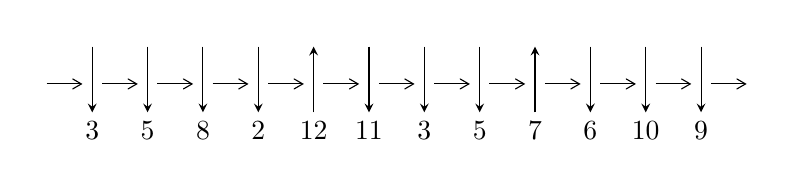
\begin{tikzpicture}[x=20pt, y=17pt]
	% nodes
	\node (C0) at (0, 0) {};
	\node (C1) at (1, 0) {};
	\node (C1U) at (1, +1) {};
	\node (C1D) at (1, -1) {3};

	\node (C2) at (2, 0) {};
	\node (C2U) at (2, +1) {};
	\node (C2D) at (2, -1) {5};

	\node (C3) at (3, 0) {};
	\node (C3U) at (3, +1) {};
	\node (C3D) at (3, -1) {8};

	\node (C4) at (4, 0) {};
	\node (C4U) at (4, +1) {};
	\node (C4D) at (4, -1) {2};

	\node (C5) at (5, 0) {};
	\node (C5U) at (5, +1) {};
	\node (C5D) at (5, -1) {12};

	\node (C6) at (6, 0) {};
	\node (C6U) at (6, +1) {};
	\node (C6D) at (6, -1) {11};

	\node (C7) at (7, 0) {};
	\node (C7U) at (7, +1) {};
	\node (C7D) at (7, -1) {3};

	\node (C8) at (8, 0) {};
	\node (C8U) at (8, +1) {};
	\node (C8D) at (8, -1) {5};

	\node (C9) at (9, 0) {};
	\node (C9U) at (9, +1) {};
	\node (C9D) at (9, -1) {7};

	\node (C10) at (10, 0) {};
	\node (C10U) at (10, +1) {};
	\node (C10D) at (10, -1) {6};

	\node (C11) at (11, 0) {};
	\node (C11U) at (11, +1) {};
	\node (C11D) at (11, -1) {10};

	\node (C12) at (12, 0) {};
	\node (C12U) at (12, +1) {};
	\node (C12D) at (12, -1) {9};
	\node (C13) at (13, 0) {};

	% arrows
	\draw[->,>={angle 60}]
	(C0) edge (C1) (C1) edge (C2) (C2) edge (C3) (C3) edge (C4) (C4) edge (C5) (C5) edge (C6) (C6) edge (C7) (C7) edge (C8) (C8) edge (C9) (C9) edge (C10) (C10) edge (C11) (C11) edge (C12) (C12) edge (C13) ;	\draw[->,>=stealth]
	(C1U) edge (C1D) (C2U) edge (C2D) (C3U) edge (C3D) (C4U) edge (C4D) (C5D) edge (C5U) (C6U) edge (C6D) (C7U) edge (C7D) (C8U) edge (C8D) (C9D) edge (C9U) (C10U) edge (C10D) (C11U) edge (C11D) (C12U) edge (C12D) ;
	\end{tikzpicture} \\
\hhline{~~} \\& 
\textbf{Solving Sequence} \\ \cline{2-2} 
 &
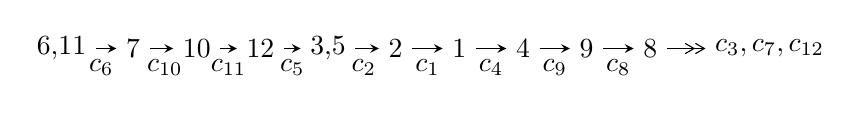
\begin{tikzpicture}[x=23pt, y=7pt]
	% node
	\node (A0) at (-1/8, 0) {6,11};
	\node (A1) at (1, 0) {7};
	\node (A2) at (2, 0) {10};
	\node (A3) at (3, 0) {12};
	\node (A4) at (65/16, 0) {3,5};
	\node (A5) at (41/8, 0) {2};
	\node (A6) at (49/8, 0) {1};
	\node (A7) at (57/8, 0) {4};
	\node (A8) at (65/8, 0) {9};
	\node (A9) at (73/8, 0) {8};
	\node (C1) at (1/2, -1) {$c_{6}$};
	\node (C2) at (3/2, -1) {$c_{10}$};
	\node (C3) at (5/2, -1) {$c_{11}$};
	\node (C4) at (7/2, -1) {$c_{5}$};
	\node (C5) at (37/8, -1) {$c_{2}$};
	\node (C6) at (45/8, -1) {$c_{1}$};
	\node (C7) at (53/8, -1) {$c_{4}$};
	\node (C8) at (61/8, -1) {$c_{9}$};
	\node (C9) at (69/8, -1) {$c_{8}$};
	\node (A10) at (11, 0) {$c_{3},c_{7},c_{12}$};

	% edge
	\draw[->,>=stealth]	
	(A0) edge (A1) (A1) edge (A2) (A2) edge (A3) (A3) edge (A4) (A4) edge (A5) (A5) edge (A6) (A6) edge (A7) (A7) edge (A8) (A8) edge (A9) ;
	\draw[->>,>={angle 60}]	
	(A9) edge (A10);
\end{tikzpicture} \\ 

\end{tabular} \\

\footnotetext{
The image of knot diagram is generated by the software ``\textbf{Draw programme}" developed by Andrew Bartholomew(\url{http://www.layer8.co.uk/maths/draw/index.htm\#Running-draw}), where we modified some parts for our purpose(\url{https://github.com/CATsTAILs/LinksPainter}).
}\phantom \\ \newline 
\centering \textbf{Ideals for irreducible components\footnotemark of $X_{\text{par}}$} 
 
\begin{align*}
I^u_{1}&=\langle 
u^{31}- u^{30}+\cdots+b-2 u,\;- u^{31}+u^{30}+\cdots+a+5 u,\;u^{32}-2 u^{31}+\cdots+5 u-1\rangle \\
I^u_{2}&=\langle 
u^6-2 u^4- u^3+u^2+b+u+1,\;u^7+u^6-2 u^5-2 u^4+u^3+u^2+a+u+1,\\
\phantom{I^u_{2}}&\phantom{= \langle  }u^9+u^8-2 u^7-3 u^6+u^5+3 u^4+2 u^3- u-1\rangle \\
\\
\end{align*}
\raggedright * 2 irreducible components of $\dim_{\mathbb{C}}=0$, with total 41 representations.\\
\footnotetext{All coefficients of polynomials are rational numbers. But the coefficients are sometimes approximated in decimal forms when there is not enough margin.}
\newpage
\renewcommand{\arraystretch}{1}
\centering \section*{I. $I^u_{1}= \langle u^{31}- u^{30}+\cdots+b-2 u,\;- u^{31}+u^{30}+\cdots+a+5 u,\;u^{32}-2 u^{31}+\cdots+5 u-1 \rangle$}
\flushleft \textbf{(i) Arc colorings}\\
\begin{tabular}{m{7pt} m{180pt} m{7pt} m{180pt} }
\flushright $a_{6}=$&$\begin{pmatrix}1\\0\end{pmatrix}$ \\
\flushright $a_{11}=$&$\begin{pmatrix}0\\u\end{pmatrix}$ \\
\flushright $a_{7}=$&$\begin{pmatrix}1\\u^2\end{pmatrix}$ \\
\flushright $a_{10}=$&$\begin{pmatrix}u\\u\end{pmatrix}$ \\
\flushright $a_{12}=$&$\begin{pmatrix}- u^3\\- u^3+u\end{pmatrix}$ \\
\flushright $a_{3}=$&$\begin{pmatrix}u^{31}- u^{30}+\cdots+8 u^2-5 u\\- u^{31}+u^{30}+\cdots-2 u^2+2 u\end{pmatrix}$ \\
\flushright $a_{5}=$&$\begin{pmatrix}u^6- u^4+1\\u^6-2 u^4+u^2\end{pmatrix}$ \\
\flushright $a_{2}=$&$\begin{pmatrix}- u^{29}+8 u^{27}+\cdots+4 u^2-2 u\\- u^{31}+u^{30}+\cdots- u^2+2 u\end{pmatrix}$ \\
\flushright $a_{1}=$&$\begin{pmatrix}- u^{11}+2 u^9-2 u^7- u^3\\- u^{13}+3 u^{11}-5 u^9+4 u^7-2 u^5- u^3+u\end{pmatrix}$ \\
\flushright $a_{4}=$&$\begin{pmatrix}u^{31}- u^{30}+\cdots+u+1\\u^{31}- u^{30}+\cdots+6 u^3- u\end{pmatrix}$ \\
\flushright $a_{9}=$&$\begin{pmatrix}u^3\\u^5- u^3+u\end{pmatrix}$ \\
\flushright $a_{8}=$&$\begin{pmatrix}u^{17}-4 u^{15}+7 u^{13}-4 u^{11}-3 u^9+6 u^7-2 u^5+u\\u^{17}-5 u^{15}+11 u^{13}-12 u^{11}+5 u^9+2 u^7-2 u^5+u\end{pmatrix}$\\&\end{tabular}
\flushleft \textbf{(ii) Obstruction class $= -1$}\\~\\
\flushleft \textbf{(iii) Cusp Shapes $= -10 u^{31}+11 u^{30}+82 u^{29}-109 u^{28}-303 u^{27}+492 u^{26}+589 u^{25}-1289 u^{24}-454 u^{23}+2036 u^{22}-559 u^{21}-1667 u^{20}+1827 u^{19}-152 u^{18}-1853 u^{17}+1907 u^{16}+315 u^{15}-1818 u^{14}+1090 u^{13}+295 u^{12}-980 u^{11}+734 u^{10}+52 u^9-568 u^8+382 u^7+24 u^6-173 u^5+145 u^4-51 u^3-48 u^2+51 u-23$}\\~\\
\newpage\renewcommand{\arraystretch}{1}
\flushleft \textbf{(iv) u-Polynomials at the component}\newline \\
\begin{tabular}{m{50pt}|m{274pt}}
Crossings & \hspace{64pt}u-Polynomials at each crossing \\
\hline $$\begin{aligned}c_{1}\end{aligned}$$&$\begin{aligned}
&u^{32}+50 u^{31}+\cdots+37 u+1
\end{aligned}$\\
\hline $$\begin{aligned}c_{2},c_{4}\end{aligned}$$&$\begin{aligned}
&u^{32}-10 u^{31}+\cdots+7 u-1
\end{aligned}$\\
\hline $$\begin{aligned}c_{3},c_{7}\end{aligned}$$&$\begin{aligned}
&u^{32}- u^{31}+\cdots+1024 u+512
\end{aligned}$\\
\hline $$\begin{aligned}c_{5},c_{9}\end{aligned}$$&$\begin{aligned}
&u^{32}+6 u^{31}+\cdots+49 u+5
\end{aligned}$\\
\hline $$\begin{aligned}c_{6},c_{10}\end{aligned}$$&$\begin{aligned}
&u^{32}+2 u^{31}+\cdots-5 u-1
\end{aligned}$\\
\hline $$\begin{aligned}c_{8}\end{aligned}$$&$\begin{aligned}
&u^{32}+2 u^{31}+\cdots-3 u-1
\end{aligned}$\\
\hline $$\begin{aligned}c_{11}\end{aligned}$$&$\begin{aligned}
&u^{32}+18 u^{31}+\cdots+9 u+1
\end{aligned}$\\
\hline $$\begin{aligned}c_{12}\end{aligned}$$&$\begin{aligned}
&u^{32}-6 u^{31}+\cdots+1421 u+145
\end{aligned}$\\
\hline
\end{tabular}\\~\\
\newpage\renewcommand{\arraystretch}{1}
\flushleft \textbf{(v) Riley Polynomials at the component}\newline \\
\begin{tabular}{m{50pt}|m{274pt}}
Crossings & \hspace{64pt}Riley Polynomials at each crossing \\
\hline $$\begin{aligned}c_{1}\end{aligned}$$&$\begin{aligned}
&y^{32}-126 y^{31}+\cdots-181 y+1
\end{aligned}$\\
\hline $$\begin{aligned}c_{2},c_{4}\end{aligned}$$&$\begin{aligned}
&y^{32}-50 y^{31}+\cdots-37 y+1
\end{aligned}$\\
\hline $$\begin{aligned}c_{3},c_{7}\end{aligned}$$&$\begin{aligned}
&y^{32}-57 y^{31}+\cdots+1310720 y+262144
\end{aligned}$\\
\hline $$\begin{aligned}c_{5},c_{9}\end{aligned}$$&$\begin{aligned}
&y^{32}+30 y^{31}+\cdots-461 y+25
\end{aligned}$\\
\hline $$\begin{aligned}c_{6},c_{10}\end{aligned}$$&$\begin{aligned}
&y^{32}-18 y^{31}+\cdots-9 y+1
\end{aligned}$\\
\hline $$\begin{aligned}c_{8}\end{aligned}$$&$\begin{aligned}
&y^{32}-66 y^{31}+\cdots-9 y+1
\end{aligned}$\\
\hline $$\begin{aligned}c_{11}\end{aligned}$$&$\begin{aligned}
&y^{32}-6 y^{31}+\cdots-17 y+1
\end{aligned}$\\
\hline $$\begin{aligned}c_{12}\end{aligned}$$&$\begin{aligned}
&y^{32}-30 y^{31}+\cdots+1291979 y+21025
\end{aligned}$\\
\hline
\end{tabular}\\~\\
\newpage\flushleft \textbf{(vi) Complex Volumes and Cusp Shapes}
$$\begin{array}{c|c|c}  
\text{Solutions to }I^u_{1}& \I (\text{vol} + \sqrt{-1}CS) & \text{Cusp shape}\\
 \hline 
\begin{aligned}
u &= \phantom{-}0.920983 + 0.401471 I \\
a &= \phantom{-}0.917136 - 1.039840 I \\
b &= \phantom{-}0.415154 + 0.155618 I\end{aligned}
 & -2.04683 - 3.28761 I & -12.15173 + 6.50570 I \\ \hline\begin{aligned}
u &= \phantom{-}0.920983 - 0.401471 I \\
a &= \phantom{-}0.917136 + 1.039840 I \\
b &= \phantom{-}0.415154 - 0.155618 I\end{aligned}
 & -2.04683 + 3.28761 I & -12.15173 - 6.50570 I \\ \hline\begin{aligned}
u &= -0.907439 + 0.255427 I \\
a &= \phantom{-}1.69960 + 1.28460 I \\
b &= \phantom{-}1.49817 + 0.96455 I\end{aligned}
 & -3.08320 + 1.04878 I & -12.81708 - 5.09104 I \\ \hline\begin{aligned}
u &= -0.907439 - 0.255427 I \\
a &= \phantom{-}1.69960 - 1.28460 I \\
b &= \phantom{-}1.49817 - 0.96455 I\end{aligned}
 & -3.08320 - 1.04878 I & -12.81708 + 5.09104 I \\ \hline\begin{aligned}
u &= -0.777091 + 0.477881 I \\
a &= -0.536566 - 0.666041 I \\
b &= -0.649263 - 0.366597 I\end{aligned}
 & \phantom{-}1.34788 + 1.99721 I & -0.92513 - 4.43380 I \\ \hline\begin{aligned}
u &= -0.777091 - 0.477881 I \\
a &= -0.536566 + 0.666041 I \\
b &= -0.649263 + 0.366597 I\end{aligned}
 & \phantom{-}1.34788 - 1.99721 I & -0.92513 + 4.43380 I \\ \hline\begin{aligned}
u &= \phantom{-}0.953782 + 0.580631 I \\
a &= -0.13862 + 2.54860 I \\
b &= -0.84091 + 1.57585 I\end{aligned}
 & -11.82200 - 5.87879 I & -11.28951 + 5.22144 I \\ \hline\begin{aligned}
u &= \phantom{-}0.953782 - 0.580631 I \\
a &= -0.13862 - 2.54860 I \\
b &= -0.84091 - 1.57585 I\end{aligned}
 & -11.82200 + 5.87879 I & -11.28951 - 5.22144 I \\ \hline\begin{aligned}
u &= \phantom{-}0.124644 + 0.870094 I \\
a &= -0.488908 - 1.119880 I \\
b &= \phantom{-}2.86386 + 0.17983 I\end{aligned}
 & -16.5159 + 6.3822 I & -11.71583 - 2.55779 I \\ \hline\begin{aligned}
u &= \phantom{-}0.124644 - 0.870094 I \\
a &= -0.488908 + 1.119880 I \\
b &= \phantom{-}2.86386 - 0.17983 I\end{aligned}
 & -16.5159 - 6.3822 I & -11.71583 + 2.55779 I\\
 \hline 
 \end{array}$$\newpage$$\begin{array}{c|c|c}  
\text{Solutions to }I^u_{1}& \I (\text{vol} + \sqrt{-1}CS) & \text{Cusp shape}\\
 \hline 
\begin{aligned}
u &= \phantom{-}0.534278 + 0.665517 I \\
a &= -1.317440 - 0.135023 I \\
b &= -1.75596 - 0.78631 I\end{aligned}
 & -10.62080 + 1.07852 I & -9.17455 + 0.26224 I \\ \hline\begin{aligned}
u &= \phantom{-}0.534278 - 0.665517 I \\
a &= -1.317440 + 0.135023 I \\
b &= -1.75596 + 0.78631 I\end{aligned}
 & -10.62080 - 1.07852 I & -9.17455 - 0.26224 I \\ \hline\begin{aligned}
u &= -1.15702\phantom{ +0.000000I} \\
a &= -2.82340\phantom{ +0.000000I} \\
b &= -1.47424\phantom{ +0.000000I}\end{aligned}
 & -16.1082\phantom{ +0.000000I} & -16.3550\phantom{ +0.000000I} \\ \hline\begin{aligned}
u &= \phantom{-}0.030254 + 0.815370 I \\
a &= \phantom{-}0.892190 + 0.010385 I \\
b &= -1.84976 - 0.76361 I\end{aligned}
 & -5.35010 + 1.73289 I & -12.16292 - 1.23498 I \\ \hline\begin{aligned}
u &= \phantom{-}0.030254 - 0.815370 I \\
a &= \phantom{-}0.892190 - 0.010385 I \\
b &= -1.84976 + 0.76361 I\end{aligned}
 & -5.35010 - 1.73289 I & -12.16292 + 1.23498 I \\ \hline\begin{aligned}
u &= \phantom{-}1.183180 + 0.412649 I \\
a &= \phantom{-}0.200378 - 0.628582 I \\
b &= \phantom{-}0.533514 + 0.079289 I\end{aligned}
 & -4.65799 - 1.98947 I & -10.09461 + 1.11362 I \\ \hline\begin{aligned}
u &= \phantom{-}1.183180 - 0.412649 I \\
a &= \phantom{-}0.200378 + 0.628582 I \\
b &= \phantom{-}0.533514 - 0.079289 I\end{aligned}
 & -4.65799 + 1.98947 I & -10.09461 - 1.11362 I \\ \hline\begin{aligned}
u &= -0.104577 + 0.739226 I \\
a &= -0.423697 + 0.357022 I \\
b &= \phantom{-}0.508988 + 0.480725 I\end{aligned}
 & -1.00221 - 1.97931 I & -5.05108 + 2.63229 I \\ \hline\begin{aligned}
u &= -0.104577 - 0.739226 I \\
a &= -0.423697 - 0.357022 I \\
b &= \phantom{-}0.508988 - 0.480725 I\end{aligned}
 & -1.00221 + 1.97931 I & -5.05108 - 2.63229 I \\ \hline\begin{aligned}
u &= -1.179880 + 0.490061 I \\
a &= \phantom{-}1.118620 - 0.044684 I \\
b &= \phantom{-}1.040940 - 0.674261 I\end{aligned}
 & -4.09969 + 6.54761 I & -8.24294 - 5.21749 I\\
 \hline 
 \end{array}$$\newpage$$\begin{array}{c|c|c}  
\text{Solutions to }I^u_{1}& \I (\text{vol} + \sqrt{-1}CS) & \text{Cusp shape}\\
 \hline 
\begin{aligned}
u &= -1.179880 - 0.490061 I \\
a &= \phantom{-}1.118620 + 0.044684 I \\
b &= \phantom{-}1.040940 + 0.674261 I\end{aligned}
 & -4.09969 - 6.54761 I & -8.24294 + 5.21749 I \\ \hline\begin{aligned}
u &= -1.222640 + 0.444091 I \\
a &= -2.70913 - 0.19363 I \\
b &= -2.46800 + 1.73197 I\end{aligned}
 & -9.06220 + 2.72579 I & -15.5836 - 2.2463 I \\ \hline\begin{aligned}
u &= -1.222640 - 0.444091 I \\
a &= -2.70913 + 0.19363 I \\
b &= -2.46800 - 1.73197 I\end{aligned}
 & -9.06220 - 2.72579 I & -15.5836 + 2.2463 I \\ \hline\begin{aligned}
u &= \phantom{-}1.218380 + 0.471883 I \\
a &= -1.38525 + 1.82670 I \\
b &= -2.45044 - 0.06343 I\end{aligned}
 & -8.86209 - 6.36925 I & -15.2047 + 4.5478 I \\ \hline\begin{aligned}
u &= \phantom{-}1.218380 - 0.471883 I \\
a &= -1.38525 - 1.82670 I \\
b &= -2.45044 + 0.06343 I\end{aligned}
 & -8.86209 + 6.36925 I & -15.2047 - 4.5478 I \\ \hline\begin{aligned}
u &= -1.257560 + 0.385869 I \\
a &= \phantom{-}2.56331 + 1.01533 I \\
b &= \phantom{-}2.30376 - 1.55155 I\end{aligned}
 & \phantom{-}18.6867 - 2.0727 I & -15.8105 - 0.3085 I \\ \hline\begin{aligned}
u &= -1.257560 - 0.385869 I \\
a &= \phantom{-}2.56331 - 1.01533 I \\
b &= \phantom{-}2.30376 + 1.55155 I\end{aligned}
 & \phantom{-}18.6867 + 2.0727 I & -15.8105 + 0.3085 I \\ \hline\begin{aligned}
u &= \phantom{-}1.223360 + 0.521615 I \\
a &= \phantom{-}2.66517 - 2.37727 I \\
b &= \phantom{-}4.04494 - 0.12748 I\end{aligned}
 & \phantom{-}19.6654 - 11.4323 I & -14.6387 + 5.6746 I \\ \hline\begin{aligned}
u &= \phantom{-}1.223360 - 0.521615 I \\
a &= \phantom{-}2.66517 + 2.37727 I \\
b &= \phantom{-}4.04494 + 0.12748 I\end{aligned}
 & \phantom{-}19.6654 + 11.4323 I & -14.6387 - 5.6746 I \\ \hline\begin{aligned}
u &= \phantom{-}0.653875\phantom{ +0.000000I} \\
a &= -0.683891\phantom{ +0.000000I} \\
b &= \phantom{-}0.233434\phantom{ +0.000000I}\end{aligned}
 & -0.923628\phantom{ +0.000000I} & -10.7930\phantom{ +0.000000I}\\
 \hline 
 \end{array}$$\newpage$$\begin{array}{c|c|c}  
\text{Solutions to }I^u_{1}& \I (\text{vol} + \sqrt{-1}CS) & \text{Cusp shape}\\
 \hline 
\begin{aligned}
u &= \phantom{-}0.511886 + 0.195210 I \\
a &= -0.803157 + 0.226384 I \\
b &= \phantom{-}0.425410 - 0.116435 I\end{aligned}
 & -0.941625 + 0.020840 I & -9.56315 + 0.03156 I \\ \hline\begin{aligned}
u &= \phantom{-}0.511886 - 0.195210 I \\
a &= -0.803157 - 0.226384 I \\
b &= \phantom{-}0.425410 + 0.116435 I\end{aligned}
 & -0.941625 - 0.020840 I & -9.56315 - 0.03156 I\\
 \hline 
 \end{array}$$\newpage\newpage\renewcommand{\arraystretch}{1}
\centering \section*{II. $I^u_{2}= \langle u^6-2 u^4- u^3+u^2+b+u+1,\;u^7+u^6-2 u^5-2 u^4+u^3+u^2+a+u+1,\;u^9+u^8-2 u^7-3 u^6+u^5+3 u^4+2 u^3- u-1 \rangle$}
\flushleft \textbf{(i) Arc colorings}\\
\begin{tabular}{m{7pt} m{180pt} m{7pt} m{180pt} }
\flushright $a_{6}=$&$\begin{pmatrix}1\\0\end{pmatrix}$ \\
\flushright $a_{11}=$&$\begin{pmatrix}0\\u\end{pmatrix}$ \\
\flushright $a_{7}=$&$\begin{pmatrix}1\\u^2\end{pmatrix}$ \\
\flushright $a_{10}=$&$\begin{pmatrix}u\\u\end{pmatrix}$ \\
\flushright $a_{12}=$&$\begin{pmatrix}- u^3\\- u^3+u\end{pmatrix}$ \\
\flushright $a_{3}=$&$\begin{pmatrix}- u^7- u^6+2 u^5+2 u^4- u^3- u^2- u-1\\- u^6+2 u^4+u^3- u^2- u-1\end{pmatrix}$ \\
\flushright $a_{5}=$&$\begin{pmatrix}u^6- u^4+1\\u^6-2 u^4+u^2\end{pmatrix}$ \\
\flushright $a_{2}=$&$\begin{pmatrix}- u^7-2 u^6+2 u^5+3 u^4- u^3- u^2- u-2\\-2 u^6+4 u^4+u^3-2 u^2- u-1\end{pmatrix}$ \\
\flushright $a_{1}=$&$\begin{pmatrix}- u^6+u^4-1\\- u^6+2 u^4- u^2\end{pmatrix}$ \\
\flushright $a_{4}=$&$\begin{pmatrix}- u^7- u^6+2 u^5+2 u^4- u^3- u^2- u-1\\- u^6+2 u^4+u^3- u^2- u-1\end{pmatrix}$ \\
\flushright $a_{9}=$&$\begin{pmatrix}u^3\\u^5- u^3+u\end{pmatrix}$ \\
\flushright $a_{8}=$&$\begin{pmatrix}1\\u^2\end{pmatrix}$\\&\end{tabular}
\flushleft \textbf{(ii) Obstruction class $= 1$}\\~\\
\flushleft \textbf{(iii) Cusp Shapes $= u^8-2 u^7- u^6+4 u^5+3 u^4-6 u^3- u^2- u-10$}\\~\\
\newpage\renewcommand{\arraystretch}{1}
\flushleft \textbf{(iv) u-Polynomials at the component}\newline \\
\begin{tabular}{m{50pt}|m{274pt}}
Crossings & \hspace{64pt}u-Polynomials at each crossing \\
\hline $$\begin{aligned}c_{1},c_{2}\end{aligned}$$&$\begin{aligned}
&(u-1)^9
\end{aligned}$\\
\hline $$\begin{aligned}c_{3},c_{7}\end{aligned}$$&$\begin{aligned}
&u^9
\end{aligned}$\\
\hline $$\begin{aligned}c_{4}\end{aligned}$$&$\begin{aligned}
&(u+1)^9
\end{aligned}$\\
\hline $$\begin{aligned}c_{5}\end{aligned}$$&$\begin{aligned}
&u^9+3 u^8+8 u^7+13 u^6+17 u^5+17 u^4+12 u^3+6 u^2+u-1
\end{aligned}$\\
\hline $$\begin{aligned}c_{6}\end{aligned}$$&$\begin{aligned}
&u^9+u^8-2 u^7-3 u^6+u^5+3 u^4+2 u^3- u-1
\end{aligned}$\\
\hline $$\begin{aligned}c_{8},c_{12}\end{aligned}$$&$\begin{aligned}
&u^9- u^8+2 u^7- u^6+3 u^5- u^4+2 u^3+u+1
\end{aligned}$\\
\hline $$\begin{aligned}c_{9}\end{aligned}$$&$\begin{aligned}
&u^9-3 u^8+8 u^7-13 u^6+17 u^5-17 u^4+12 u^3-6 u^2+u+1
\end{aligned}$\\
\hline $$\begin{aligned}c_{10}\end{aligned}$$&$\begin{aligned}
&u^9- u^8-2 u^7+3 u^6+u^5-3 u^4+2 u^3- u+1
\end{aligned}$\\
\hline $$\begin{aligned}c_{11}\end{aligned}$$&$\begin{aligned}
&u^9+5 u^8+12 u^7+15 u^6+9 u^5- u^4-4 u^3-2 u^2+u+1
\end{aligned}$\\
\hline
\end{tabular}\\~\\
\newpage\renewcommand{\arraystretch}{1}
\flushleft \textbf{(v) Riley Polynomials at the component}\newline \\
\begin{tabular}{m{50pt}|m{274pt}}
Crossings & \hspace{64pt}Riley Polynomials at each crossing \\
\hline $$\begin{aligned}c_{1},c_{2},c_{4}\end{aligned}$$&$\begin{aligned}
&(y-1)^9
\end{aligned}$\\
\hline $$\begin{aligned}c_{3},c_{7}\end{aligned}$$&$\begin{aligned}
&y^9
\end{aligned}$\\
\hline $$\begin{aligned}c_{5},c_{9}\end{aligned}$$&$\begin{aligned}
&y^9+7 y^8+20 y^7+25 y^6+5 y^5-15 y^4+22 y^2+13 y-1
\end{aligned}$\\
\hline $$\begin{aligned}c_{6},c_{10}\end{aligned}$$&$\begin{aligned}
&y^9-5 y^8+12 y^7-15 y^6+9 y^5+y^4-4 y^3+2 y^2+y-1
\end{aligned}$\\
\hline $$\begin{aligned}c_{8},c_{12}\end{aligned}$$&$\begin{aligned}
&y^9+3 y^8+8 y^7+13 y^6+17 y^5+17 y^4+12 y^3+6 y^2+y-1
\end{aligned}$\\
\hline $$\begin{aligned}c_{11}\end{aligned}$$&$\begin{aligned}
&y^9- y^8+12 y^7-7 y^6+37 y^5+y^4-10 y^2+5 y-1
\end{aligned}$\\
\hline
\end{tabular}\\~\\
\newpage\flushleft \textbf{(vi) Complex Volumes and Cusp Shapes}
$$\begin{array}{c|c|c}  
\text{Solutions to }I^u_{2}& \I (\text{vol} + \sqrt{-1}CS) & \text{Cusp shape}\\
 \hline 
\begin{aligned}
u &= -0.772920 + 0.510351 I \\
a &= -0.147032 - 1.012940 I \\
b &= -0.848670 - 0.225310 I\end{aligned}
 & \phantom{-}0.13850 + 2.09337 I & -9.40455 - 4.13635 I \\ \hline\begin{aligned}
u &= -0.772920 - 0.510351 I \\
a &= -0.147032 + 1.012940 I \\
b &= -0.848670 + 0.225310 I\end{aligned}
 & \phantom{-}0.13850 - 2.09337 I & -9.40455 + 4.13635 I \\ \hline\begin{aligned}
u &= \phantom{-}0.825933\phantom{ +0.000000I} \\
a &= -1.95176\phantom{ +0.000000I} \\
b &= -1.33142\phantom{ +0.000000I}\end{aligned}
 & -2.84338\phantom{ +0.000000I} & -12.5800\phantom{ +0.000000I} \\ \hline\begin{aligned}
u &= \phantom{-}1.173910 + 0.391555 I \\
a &= \phantom{-}0.679689 + 0.626017 I \\
b &= \phantom{-}0.25695 + 1.39155 I\end{aligned}
 & -6.01628 - 1.33617 I & -15.1179 + 0.3856 I \\ \hline\begin{aligned}
u &= \phantom{-}1.173910 - 0.391555 I \\
a &= \phantom{-}0.679689 - 0.626017 I \\
b &= \phantom{-}0.25695 - 1.39155 I\end{aligned}
 & -6.01628 + 1.33617 I & -15.1179 - 0.3856 I \\ \hline\begin{aligned}
u &= -0.141484 + 0.739668 I \\
a &= -0.541407 + 0.753907 I \\
b &= \phantom{-}0.443165 - 0.284059 I\end{aligned}
 & -2.26187 - 2.45442 I & -10.97405 + 3.19656 I \\ \hline\begin{aligned}
u &= -0.141484 - 0.739668 I \\
a &= -0.541407 - 0.753907 I \\
b &= \phantom{-}0.443165 + 0.284059 I\end{aligned}
 & -2.26187 + 2.45442 I & -10.97405 - 3.19656 I \\ \hline\begin{aligned}
u &= -1.172470 + 0.500383 I \\
a &= \phantom{-}0.484630 + 0.655708 I \\
b &= \phantom{-}1.314260 + 0.168567 I\end{aligned}
 & -5.24306 + 7.08493 I & -14.2133 - 6.7157 I \\ \hline\begin{aligned}
u &= -1.172470 - 0.500383 I \\
a &= \phantom{-}0.484630 - 0.655708 I \\
b &= \phantom{-}1.314260 - 0.168567 I\end{aligned}
 & -5.24306 - 7.08493 I & -14.2133 + 6.7157 I\\
 \hline 
 \end{array}$$\newpage
\newpage\renewcommand{\arraystretch}{1}
\centering \section*{ III. u-Polynomials}
\begin{tabular}{m{50pt}|m{274pt}}
Crossings & \hspace{64pt}u-Polynomials at each crossing \\
\hline $$\begin{aligned}c_{1}\end{aligned}$$&$\begin{aligned}
&((u-1)^9)(u^{32}+50 u^{31}+\cdots+37 u+1)
\end{aligned}$\\
\hline $$\begin{aligned}c_{2}\end{aligned}$$&$\begin{aligned}
&((u-1)^9)(u^{32}-10 u^{31}+\cdots+7 u-1)
\end{aligned}$\\
\hline $$\begin{aligned}c_{3},c_{7}\end{aligned}$$&$\begin{aligned}
&u^9(u^{32}- u^{31}+\cdots+1024 u+512)
\end{aligned}$\\
\hline $$\begin{aligned}c_{4}\end{aligned}$$&$\begin{aligned}
&((u+1)^9)(u^{32}-10 u^{31}+\cdots+7 u-1)
\end{aligned}$\\
\hline $$\begin{aligned}c_{5}\end{aligned}$$&$\begin{aligned}
&(u^9+3 u^8+8 u^7+13 u^6+17 u^5+17 u^4+12 u^3+6 u^2+u-1)\\
&\cdot(u^{32}+6 u^{31}+\cdots+49 u+5)
\end{aligned}$\\
\hline $$\begin{aligned}c_{6}\end{aligned}$$&$\begin{aligned}
&(u^9+u^8+\cdots- u-1)(u^{32}+2 u^{31}+\cdots-5 u-1)
\end{aligned}$\\
\hline $$\begin{aligned}c_{8}\end{aligned}$$&$\begin{aligned}
&(u^9- u^8+\cdots+u+1)(u^{32}+2 u^{31}+\cdots-3 u-1)
\end{aligned}$\\
\hline $$\begin{aligned}c_{9}\end{aligned}$$&$\begin{aligned}
&(u^9-3 u^8+8 u^7-13 u^6+17 u^5-17 u^4+12 u^3-6 u^2+u+1)\\
&\cdot(u^{32}+6 u^{31}+\cdots+49 u+5)
\end{aligned}$\\
\hline $$\begin{aligned}c_{10}\end{aligned}$$&$\begin{aligned}
&(u^9- u^8+\cdots- u+1)(u^{32}+2 u^{31}+\cdots-5 u-1)
\end{aligned}$\\
\hline $$\begin{aligned}c_{11}\end{aligned}$$&$\begin{aligned}
&(u^9+5 u^8+12 u^7+15 u^6+9 u^5- u^4-4 u^3-2 u^2+u+1)\\
&\cdot(u^{32}+18 u^{31}+\cdots+9 u+1)
\end{aligned}$\\
\hline $$\begin{aligned}c_{12}\end{aligned}$$&$\begin{aligned}
&(u^9- u^8+2 u^7- u^6+3 u^5- u^4+2 u^3+u+1)\\
&\cdot(u^{32}-6 u^{31}+\cdots+1421 u+145)
\end{aligned}$\\
\hline
\end{tabular}\newpage\renewcommand{\arraystretch}{1}
\centering \section*{ IV. Riley Polynomials}
\begin{tabular}{m{50pt}|m{274pt}}
Crossings & \hspace{64pt}Riley Polynomials at each crossing \\
\hline $$\begin{aligned}c_{1}\end{aligned}$$&$\begin{aligned}
&((y-1)^9)(y^{32}-126 y^{31}+\cdots-181 y+1)
\end{aligned}$\\
\hline $$\begin{aligned}c_{2},c_{4}\end{aligned}$$&$\begin{aligned}
&((y-1)^9)(y^{32}-50 y^{31}+\cdots-37 y+1)
\end{aligned}$\\
\hline $$\begin{aligned}c_{3},c_{7}\end{aligned}$$&$\begin{aligned}
&y^9(y^{32}-57 y^{31}+\cdots+1310720 y+262144)
\end{aligned}$\\
\hline $$\begin{aligned}c_{5},c_{9}\end{aligned}$$&$\begin{aligned}
&(y^9+7 y^8+20 y^7+25 y^6+5 y^5-15 y^4+22 y^2+13 y-1)\\
&\cdot(y^{32}+30 y^{31}+\cdots-461 y+25)
\end{aligned}$\\
\hline $$\begin{aligned}c_{6},c_{10}\end{aligned}$$&$\begin{aligned}
&(y^9-5 y^8+12 y^7-15 y^6+9 y^5+y^4-4 y^3+2 y^2+y-1)\\
&\cdot(y^{32}-18 y^{31}+\cdots-9 y+1)
\end{aligned}$\\
\hline $$\begin{aligned}c_{8}\end{aligned}$$&$\begin{aligned}
&(y^9+3 y^8+8 y^7+13 y^6+17 y^5+17 y^4+12 y^3+6 y^2+y-1)\\
&\cdot(y^{32}-66 y^{31}+\cdots-9 y+1)
\end{aligned}$\\
\hline $$\begin{aligned}c_{11}\end{aligned}$$&$\begin{aligned}
&(y^9- y^8+12 y^7-7 y^6+37 y^5+y^4-10 y^2+5 y-1)\\
&\cdot(y^{32}-6 y^{31}+\cdots-17 y+1)
\end{aligned}$\\
\hline $$\begin{aligned}c_{12}\end{aligned}$$&$\begin{aligned}
&(y^9+3 y^8+8 y^7+13 y^6+17 y^5+17 y^4+12 y^3+6 y^2+y-1)\\
&\cdot(y^{32}-30 y^{31}+\cdots+1291979 y+21025)
\end{aligned}$\\
\hline
\end{tabular}
\vskip 2pc
\end{document}